\chapter{Measurement of Mass and Position of Center of Mass of the Frame }\label{app:MassFrameCenterOfMass} 
\textbf{Name: Group 630}\\
\textbf{Date: 15/03 - 2016}

\subsubsection{Purpose}
Measure the mass and center of mass of the frame.

\subsubsection{List of Equipment}
\begin{table}[H]
	\begin{tabular}{|l|l|p{4.3cm}|}
		\hline%------------------------------------------------------------------------------------------------------------
		\textbf{Instrument}                                  &  \textbf{AAU-no.}  &  \textbf{Type}                       \\
		\hline%------------------------------------------------------------------------------------------------------------
		Scale                                           & 86759            &  		                   \\
		\hline%------------------------------------------------------------------------------------------------------------
		Dedicated Power Supply of Cubli \small{(24 V - 3 A)} &  AAU3                   &  XP Power, AEB70US24                 \\
		\hline%------------------------------------------------------------------------------------------------------------
		Digital Protractor                                   &  None               & CMT Orange Tools     \\
		\hline%------------------------------------------------------------------------------------------------------------
	\end{tabular}
\end{table}
\subsubsection{Procedure}
\begin{enumerate}
	\item The Cubli base frame is leveled and the angle of equilibrium point is measured.
	\item The frame is dismounted from the base and weight.
	\item The frame is mounted back on the base after being rotated 90 degrees and the angle of equilibrium point is measured.
	\item The Cubli frame is returned to the original placement on the base frame.
\end{enumerate}


\subsubsection{Results of the frame weight}
\begin{table}[H]
	\begin{tabular}{|l|l|p{4.3cm}|}
		\hline%------------------------------------------------------------------------------------------------------------
		\textbf{Weight of the frame}       &  \textbf{kg}         \\
		\hline%------------------------------------------------------------------------------------------------------------
		Fully mounted frame        	  & 0,770          \\
		\hline%------------------------------------------------------------------------------------------------------------
		Mass of the wheel        	  & 0,222          \\
		\hline%------------------------------------------------------------------------------------------------------------
	\end{tabular}
\end{table}	
By subtracting the known mass of the wheel form the fully mounted frame, it gives a frame mass of \si{0,548\ kg}.

\subsubsection{Results of center of mass}
To measure the center of mass the equilibrium positions of the frame on sides that are orthogonal must be determined. They can be seen in \figref{centerOfMassDiagram2}, and the total center correspond to the crossing of the two lines.
\begin{table}[H]
	\begin{tabular}{|l|l|p{5cm}|}
		\hline%------------------------------------------------------------------------------------------------------------
		\textbf{Frame rotation angle}       &  \textbf{Angle from equilibrium point}       &  \textbf{Converted angle} \\
		\hline%------------------------------------------------------------------------------------------------------------
		\si{0^{\circ}}       & \si{2,5^{\circ}}      & \SI{0,043}{rad}     \\
		\hline%------------------------------------------------------------------------------------------------------------
		\si{90^{\circ}} 	 & \si{4,5^{\circ}}   & \SI{0,078}{rad}   \\
		\hline%------------------------------------------------------------------------------------------------------------
	\end{tabular}
\end{table}

\begin{figure}[H]
	\centering
	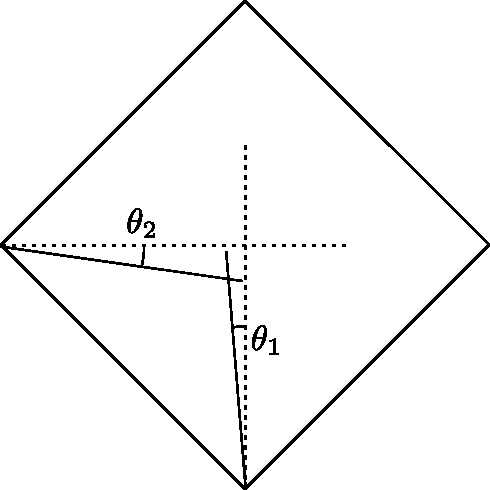
\includegraphics[scale=0.5]{figures/centerOfMassDiagram}
	\caption{Location of the center of mass, where \si{\theta_1=0,043\ rad\ and\ \theta_2=0,078\ rad}}
	\label{centerOfMassDiagram2}
\end{figure}